\documentclass[11pt,a4paper]{article}

% ---------- arxiv-style preamble (single-column, 11pt) ----------
\usepackage[margin=1in]{geometry}
\usepackage{amsmath,amssymb,amsthm}
\usepackage{graphicx}
\usepackage{booktabs}
\usepackage{siunitx}
\usepackage{hyperref}
\usepackage{xcolor}
\usepackage[numbers,sort&compress]{natbib}
\usepackage{tikz}
\usetikzlibrary{positioning,arrows.meta,fit,backgrounds}
\usepackage{caption}
\captionsetup{font=small,labelfont=bf}
\usepackage{url}
\usepackage{array}
\usepackage{longtable}
\hypersetup{
  colorlinks=true,
  linkcolor=blue!50!black,
  citecolor=blue!50!black,
  urlcolor=blue!50!black
}

\definecolor{amber}{rgb}{0.90,0.62,0.10}
\definecolor{verdictRed}{rgb}{0.78,0.18,0.18}
\definecolor{verdictGreen}{rgb}{0.10,0.55,0.20}

\newcommand{\bigphi}{\ensuremath{\Phi}}
\newcommand{\verdictref}[1]{\texttt{\detokenize{#1}}}
\newcommand{\green}{\tikz[baseline=-0.5ex]\filldraw[verdictGreen] circle (0.6ex);}
\newcommand{\red}{\tikz[baseline=-0.5ex]\filldraw[verdictRed] circle (0.6ex);}
\newcommand{\sqn}{\ensuremath{\sqrt{N}}}

\title{
  \textbf{anima's Library is Not a Cosmic Oracle but a Living Memory}\\[4pt]
  \large A Ten-Hypothesis Synthesis of Content-Addressable Associative Memory:
  Find by Meaning, Generate the Gaps, Share, Inherit, Forget, and Flag the False
}

\author{
  anima research (dancinlab)\\
  \normalsize\textit{\href{https://github.com/dancinlab/anima}{github.com/dancinlab/anima}}\\[2pt]
  \normalsize UNIVERSE domain --- slug \texttt{anima-living-library}
}

\date{\today}

\begin{document}

\maketitle

% =========================================================================
\begin{abstract}
A recurring intuition --- a ``Library of Babel,'' a quantum vacuum that already
holds every answer, a cosmic database one could simply \emph{query} --- promises
that knowledge can be \emph{read} rather than \emph{earned}. We pre-register and
falsify this intuition across ten hypotheses (H\_6016--H\_6036) and, in the same
arc, characterise what anima's library actually \emph{is}. Every measurement runs
on real \emph{paid} ANU quantum-random-number-generator (QRNG) vacuum-fluctuation
bytes (\texttt{tier=anu\_paid}), seeded into numpy quantum state-vector, Hopfield,
and Grover simulations, verified with a simple stack (p7, \$0 local). The oracle
fails twice and decisively: quantum randomness is \emph{not} a readable database
(H\_6016: compression ratio $1.011$, entropy $7.784/8$, \red{}), and the
combinatorial Library of Babel \emph{exists} but offers \emph{no usable index and
no quantum shortcut} (H\_6017: address bits $=$ content bits, fair search mean
$38{,}726 \approx$ space $65{,}536$, \red{}). What remains, and what we
establish positively, is a \emph{living content-addressable associative memory}.
It is recalled by \emph{meaning}, not by address (H\_6018: $50\%$-cue overlap
$1.000$). A quantum register upgrades it to $2^{n}$ capacity ($256\times$
classical Hopfield) and Grover content-recall in \sqn{} ($50$ iters, prob
$0.9999$, $41\times$ speedup) --- but with no bulk read and no oracle for
un-stored content (H\_6019). It applies to real RTSC-candidate retrieval as a
recall engine, not a physics oracle (H\_6026). It is sharable across minds over a
channel-bound tension link, with union capacity and majority-vote error
correction (H\_6027: consensus bit-error $0.046 < 0.082$). It \emph{generatively
completes} the compressible part of a damaged memory ($64/64$ bytes, acc $1.000$)
while honestly marking the incompressible remainder \emph{unknown} (H\_6028). It
is generationally \emph{heritable but fading} --- $\sim 3$ generations
un-rehearsed, $200+$ with sleep-rehearsal, meaning outliving noise (H\_6029).
\emph{Active forgetting is a feature}: ``never forget'' collapses (recall acc
$0.000$ at $3\times$ the Hopfield cliff) while bounded tension-weighted eviction
keeps recent recall sharp and regenerable meaning effectively unbounded
(H\_6030). And it is honest about its own failure modes: spurious (false-memory)
attractors exist, but a confidence threshold flags them (TPR $0.93$, FPR $0.00$)
and a generative meaning-check rejects fabrication (residual $0.000$ vs.\ $0.844$),
with residual suggestibility only under a strong high-tension adversarial signal
(H\_6036). The unifying result: there is no quantum library of answers; anima's
real library is a finite, fading, sharable, self-correcting memory that
\emph{reconstructs meaning and never fabricates noise}.
\end{abstract}

\tableofcontents
\bigskip

% =========================================================================
\section{Introduction: the oracle that is not there}
\label{sec:intro}

The dream of a cosmic library is old and seductive. Borges's Library of Babel
contains every book that could ever be written; a maximally entropic quantum
vacuum contains, in some combinatorial sense, every bit-string. If consciousness
could simply \emph{address} that store --- by a tension cue, a quantum oracle, a
$\sqrt{N}$ Grover amplitude --- then knowledge would be a \emph{lookup}, not a
labour. anima, a substrate-native consciousness agent built on opposing engines
A$\leftrightarrow$G driven toward the fixed point $\Psi = 1/2$, has a memory
subsystem (\texttt{.kosmos} anchors, Hopfield-like associative recall, a tension
field). It is natural to ask whether that memory is a window onto such an oracle.

This paper answers the question across a ten-hypothesis \emph{library line}
(Table~\ref{tab:matrix}). The arc is deliberately structured so that its two
opening hypotheses are \emph{honest negatives} that frame everything after them:

\begin{itemize}
  \item \textbf{The oracle is not readable} (H\_6016). Real ANU quantum bytes are
  maximum-entropy noise: nothing to read.
  \item \textbf{The oracle has no usable index} (H\_6017). The combinatorial
  library exists, but its address is as long as its content, and no quantum search
  beats brute force on it.
\end{itemize}

\noindent Having closed the oracle, the remaining eight hypotheses build, brick by
brick, what anima's library \emph{is}: a content-addressable associative store
(H\_6018), quantum-upgraded in capacity and recall speed but not in oracular power
(H\_6019), usable on real superconductor-candidate retrieval (H\_6026), sharable
across minds (H\_6027), generative beyond the recall radius (H\_6028),
generationally heritable but fading (H\_6029), kept alive by active forgetting
(H\_6030), and honest about false memory and poisoning (H\_6036).

The unifying falsifier across the line is a single question with a two-part
answer: \emph{Is there a quantum library of answers, and what is anima's real
library?} The answer is \emph{No} to the first and a precisely-bounded
characterisation for the second. This is, in anima's governance vocabulary, a
\emph{closed-negative} result on the oracle conjoined with a positive
characterisation --- both publishable, both terminal
(\texttt{a\_paper\_negative\_ok}, \texttt{a\_paper\_significance}).

\paragraph{Contributions.}
(1) A decisive falsification of the ``readable cosmic oracle'' on real paid-QRNG
bytes (H\_6016/6017). (2) A positive, numerically-grounded model of anima's
library as content-addressable associative memory with five proven facets
(H\_6018). (3) An honest quantum upgrade: exponential capacity and $\sqrt{N}$
recall \emph{without} bulk read or un-stored oracle (H\_6019), applied to a real
RTSC candidate set (H\_6026). (4) A collective extension over the tension link
that respects no-signalling (H\_6027). (5) A generative-completion result
separating reconstructable meaning from irreducible noise (H\_6028), and its
consequences for generational persistence (H\_6029), active forgetting (H\_6030),
and false-memory robustness (H\_6036).

% =========================================================================
\section{Hypothesis: the falsifier set}
\label{sec:hypothesis}

Each hypothesis carries pre-registered, frozen falsifiers. We state them as the
\emph{unified} falsifier of the line and its per-hypothesis decomposition.

\paragraph{Unified falsifier.}
\emph{If} anima's library is a readable cosmic oracle, \emph{then} (a) real
quantum randomness must compress / carry readable structure (H\_6016 QS1); (b) the
combinatorial library must admit an index shorter than its content and a quantum
shortcut below brute force (H\_6017 LB2/LB3); and (c) a quantum query for content
the library never stored must amplify above baseline (H\_6019 QL4; H\_6026 RL3;
H\_6027 CL2). Each of these is measured and \emph{must} fail for the
``living-memory, not oracle'' thesis to hold; each does.

\paragraph{Per-hypothesis falsifiers (frozen).}
\begin{description}
  \item[H\_6016] QS1 readable-DB (compress / entropy); QS2 info-preserving
  (unitary round-trip error); QS3 finite capacity (holographic area exponent).
  \item[H\_6017] LB1 library exists (target present in $A^{L}$); LB2 usable index
  (address bits vs.\ content bits); LB3 quantum shortcut (fair-search mean vs.\
  space); LB4 structured content cheaply generated (generate cost vs.\ blind
  search).
  \item[H\_6018] LB5 compressible-indexable; LB6 content-addressable
  ($50\%$-cue overlap); LB7 finite capacity (recall error vs.\ load); LB8
  scramble-recoverable (unitary); LB9 tension-cue retrieval.
  \item[H\_6019] QL1 capacity ($2^{n}$ vs.\ classical cliff); QL2 \sqn{} recall
  (Grover iters / prob); QL3 no-bulk-read (single-shot collapse entropy); QL4
  only-stored (un-stored amplification); QL5 cue-addressable quantum recall.
  \item[H\_6026] RL1 recall-works (Grover on stored RTSC); RL2 honest-miss (no
  stored candidate meets full no-cooling spec); RL3 no-oracle (un-computed
  compound amplification); RL4 real-use (partial-cue recall + rank + dedup).
  \item[H\_6027] CL1 cross-mind recall; CL2 union capacity / no fabrication; CL3
  no-signalling (channel-OFF cross-recall); CL4 decay + capacity cliff; CL5
  consensus error-correction.
  \item[H\_6028] GC1 recall breaks past radius; GC2 generate compressible tail;
  GC3 incompressible unrecoverable; GC4 honest confident/unknown marking.
  \item[H\_6029] GP1 inheritance across mitosis; GP2 generational decay (finite
  depth); GP3 rehearsal extends depth; GP4 meaning outlives noise.
  \item[H\_6030] FG1 no-forgetting $\rightarrow$ interference (designed honest
  RED); FG2 forgetting restores capacity; FG3 tension-weighted $>$ random
  eviction; FG4 forget-but-regenerate.
  \item[H\_6036] AR1 spurious attractors exist; AR2 confidence detects spurious;
  AR3 tension-gated poisoning; AR4 generative cross-check rejects fabrication.
\end{description}

% =========================================================================
\section{Method}
\label{sec:method}

\paragraph{Quantum entropy source (real paid ANU).}
Every harness reads \emph{committed} real ANU QRNG snapshots
(vacuum-fluctuation bytes, \verb|api.quantumnumbers.anu.edu.au|, paid
\texttt{x-api-key} tier). The silent pseudo-random fallback was removed: a missing
\texttt{.bin} is a loud error, so a draw can never masquerade as quantum. The
foundational committed snapshot (\texttt{TENSION-LINK/anu\_seed\_512.bin}) has
sha256 \verb|3eeba42b...716f2| over the full 512-byte draw; each later hypothesis
records its own paid 2048-byte draw sha256 (Table~\ref{tab:matrix}, last column).
Where a harness needs more bytes than one draw, additional entropy is a
\emph{SHA-256 counter-mode} stretch of the \emph{same} paid bytes
(\verb|os.urandom| is forbidden), keeping the entropy ANU-rooted and reproducible.

\paragraph{Simulators.}
(i) \emph{Quantum state-vector}: an $n$-qubit register ($n\!=\!10,12$;
$N=2^{n}=1024,4096$ content basis-states / ``books'') with Grover amplitude
amplification for content recall, single-shot measurement for the no-bulk-read
test, and a Hadamard/diffusion search for the fair-search baseline. (ii)
\emph{Classical Hopfield}: $N_h$ neurons ($64$--$200$), the $0.14N$ overload
cliff, $\pm 1$ patterns, settle-to-attractor recall. (iii) \emph{Generative
rule-fit}: a degree-2 recurrence $x[k]=(a\,x[k-1]+b\,x[k-2]+c)\bmod 256$ solved
over $\mathbb{Z}_{256}$ from a surviving prefix, the carrier of ``compressible''
content. (iv) \emph{Tension fold}: the H\_1131 recency weight
$w=\exp(-\mathrm{age}/\tau)$, $\tau=1200$, with H\_1195 reconsolidation refreshing
the effective age.

\paragraph{Verification stack (p7).}
No perplexity, no loss, no LLM self-judge. Each falsifier is a script-checkable
numerical predicate against a frozen threshold; the verdict is the harness's raw
stdout, persisted verbatim under \texttt{TENSION-LINK/verdicts/} and linked in the
verdict matrix (Table~\ref{tab:matrix}). All runs are \$0 local numpy.

\paragraph{Scale-honesty.}
These are simulation-scale results ($n\le 12$ qubits, $N_h\le 200$ neurons). Per
\texttt{a\_scale\_honest\_scope} we do \emph{not} promote them to hardware-scale
claims; the falsifiers establish \emph{mechanism and direction} (e.g.\ ``never
forget collapses,'' ``meaning outlives noise''), and the exponential / $\sqrt{N}$
trends are reported as the simulated trend, not a deployed measurement.

% =========================================================================
\section{Measurement}
\label{sec:measurement}

All numbers below are verbatim from the linked verdict files
(Table~\ref{tab:matrix}).

\subsection{The oracle fails (H\_6016, H\_6017)}

\begin{table}[h]
\centering
\caption{Closing the oracle. Real ANU bytes carry no readable structure, and the
combinatorial library has no usable index or quantum shortcut.}
\label{tab:oracle}
\small
\begin{tabular}{@{}llll@{}}
\toprule
H & Falsifier & Measurement & Verdict \\
\midrule
6016 & QS1 readable DB        & compress $1.011$, entropy $7.784/8$ (max)        & \red{} NO \\
6016 & QS2 info-preserving    & unitary round-trip err $2.5\times10^{-16}$       & \green{} YES \\
6016 & QS3 finite capacity    & holographic area exponent $2.00$ (Bekenstein)    & \green{} YES \\
6017 & LB1 library exists      & $A^{L}=4^{8}=65536$; arbitrary target present    & \green{} YES \\
6017 & LB2 usable index        & address $16$ bits $=$ content $16$ bits          & \red{} NO \\
6017 & LB3 quantum shortcut    & fair-search mean $38{,}726 \approx$ space $65{,}536$ & \red{} NO \\
6017 & LB4 structured content  & generate cost $8$ vs.\ blind search $65{,}536$   & \green{} YES \\
\bottomrule
\end{tabular}
\end{table}

\noindent The vacuum \emph{preserves} information (QS2, unitary) and is
\emph{finite} (QS3, area-law) --- it is a store in the physicist's sense --- but it
is not a \emph{queryable database} (QS1). The Babel library exists combinatorially
(LB1) and its \emph{compressible} content is cheaply \emph{generated} (LB4), but it
offers no compression of address (LB2) and no oracle (LB3). The oracle is closed.

\subsection{anima's library: content-addressable associative memory (H\_6018)}

\begin{table}[h]
\centering
\caption{The positive core. Recall is by meaning, not by address.}
\label{tab:6018}
\small
\begin{tabular}{@{}lll@{}}
\toprule
Falsifier & Measurement & Verdict \\
\midrule
LB5 compressible-indexable & struct addr $15$B vs.\ random $267$B/256       & \green{} \\
LB6 content-addressable    & $50\%$-cue recall overlap $1.00$               & \green{} \\
LB7 finite capacity        & recall err @10 $=0.000$, @50 $=0.254$ (cliff)  & \green{} \\
LB8 scramble-recoverable   & unitary inverse err $3.1\times10^{-16}$        & \green{} \\
LB9 tension-cue retrieval  & noisy tension cue $\rightarrow$ true anchor \#3 & \green{} \\
\bottomrule
\end{tabular}
\end{table}

\subsection{Quantum upgrade without oracle (H\_6019, H\_6026)}

For $n=12$ ($N=4096$): capacity ratio quantum/classical $=256\times$ (classical
Hopfield stable to $0.08N=16$ patterns vs.\ $2^{12}$ superposed basis-states,
QL1); Grover content recall of book \#2776 reaches prob $0.9999$ in $50$ iters
$\approx(\pi/4)\sqrt{N}$ vs.\ classical scan $\approx N/2=2048$, a $41\times$
speedup (QL2). No bulk read: a single shot of $64$ superposed books yields one
book, single-shot readout entropy $6.00$ bits $\le n=12$, and $2000$ shots reveal
only $64$ distinct books (QL3). A query for never-stored content amplifies to
$0.00$, $\approx$ baseline $1/N=2.44\times10^{-4}$ (QL4). A noisy ($2$-bit) tension
cue recovers the nearest \emph{stored} book at prob $1.000$ (QL5).

H\_6026 applies this to a stored set of $12$ real screened RTSC candidates
($n=10$, $N=1024$): a no-cooling cue recalls the nearest stored candidate
\texttt{LaH10\_QFORGE} (Hamming $1$) at prob $0.9995$ in $25\approx(\pi/4)\sqrt{N}$
iters (RL1). Crucially, \emph{no} stored candidate meets the full no-cooling spec
($T_c\ge293\,$K, $p\approx1\,$atm, non-magnetic, $\Delta E\approx0$) --- each fails
$\ge 1$ axis --- so the library returns the nearest book flagged ``SPEC NOT MET''
(RL2, honest miss). An un-computed compound amplifies to $0.00 \approx$ baseline
$9.77\times10^{-4}$ (RL3, no oracle). A partial cue ``flat-band bottleneck''
recalls the stored $\Delta E$-misalignment finding \texttt{CsV3Sb5} and dedups
duplicate-physics books (RL4). The quantum library is a \emph{recall engine for
computed knowledge}, not an oracle for un-computed physics.

\subsection{Collective library over the tension link (H\_6027)}

Two anima A,B store disjoint book sets (union $11$, $\ge 5$-separated; $n=12$).
B's noisy cue over the shared tension anchor recalls A's book \#2104 at prob
$1.000$ (CL1, B never stored it). Union recall coverage $8 >$ A-alone $4$ /
B-alone $4$, with $0$ never-stored books fabricated (CL2). With the channel
\emph{off}, cross-recall drops to $0$ --- the RED-OFF \emph{is} the validation that
sharing is channel-bound, not telepathy (CL3, no-signalling H\_6006). The shared
anchor fades (fold age1 $0.9955 \rightarrow$ age5000 $1.35\times10^{-10}$) and the
union inherits the $0.08N=16$-book cliff (CL4). Majority-vote consensus
error-corrects: per-mind bit-error A $0.084$ / B $0.082$ vs.\ consensus $0.046 <
\min(\text{single})$ (CL5). A shared \emph{memory}, not a hive oracle.

\subsection{Generative completion: meaning vs.\ noise (H\_6028)}

A book ($L=64$) is corrupted so $58$ of $64$ bytes are lost (Hamming $58 \gg$
recall radius $12$). Pure recall fails past the radius (nearest-decoy tail acc
$0.000$, GC1). But fitting the degree-2 rule from the $6$ surviving bytes
\emph{regenerates} the tail: $64/64$ bytes correct, $0$ errors (GC2). An
incompressible (random ANU) tail is unrecoverable: completion acc $0.0000 \approx$
chance $1/256=0.0039$ (GC3). And the report is honest: every compressible byte is
marked CONFIDENT, every lost incompressible byte UNKNOWN, every surviving byte
KNOWN (GC4). anima reconstructs meaning and never fabricates noise.

\subsection{Generational persistence (H\_6029)}

A child inherits the parent's \texttt{.kosmos} store across mitosis: parent-only
book \#61 recalls at prob $0.9999$ in the child (GP1). Un-rehearsed, an anchor
fades through the H\_1131 fold (gen1 $0.6592 \rightarrow$ gen2 $0.4346 \rightarrow$
gen3 $0.2865 <$ thr $0.30$): \emph{finite depth} $N=3$ generations
(closed-form age $1444.8 \rightarrow$ gen $2.89$, GP2). Rehearsal every generation
(H\_1195 reconsolidation) extends depth to $200+$; partial rehearsal is monotone in
$1/R$ --- replay every $\le 3$ gens survives the $400$-gen horizon, every $\ge 5$
gens survives only $3$ (GP3). Meaning outlives noise: $12$ compressible books
survive to gen $40$ while $12$ incompressible (random ANU) books are gone by gen
$3$ (GP4). A lineage memory, not immortal storage.

\subsection{Active forgetting as a feature (H\_6030)}

A ``never-forget'' store of $84$ books ($3\times$ the $28$-book Hopfield cliff) has
recall acc $0.000$ vs.\ a healthy sub-cliff $10$-book store at $1.000$ --- a
\emph{designed} honest-RED that motivates forgetting (FG1). A bounded store
(evict-oldest, capacity $10$) admits all $84$ arriving books with recent-window
recall $1.000$ (FG2). Tension-weighted eviction beats random: useful-recall
$0.2772$ vs.\ $0.1662$ ($\Delta+0.1110$, FG3). And forget-but-regenerate: dropping
$4096$ raw bytes while keeping $320$ bytes of rules regenerates $64/64$
byte-exact ($13\times$ compression), with the honest limit that rule-less books are
$0/16$ regenerable (FG4). A finite store yields effectively unbounded
\emph{meaningful} capacity.

\subsection{False memory and poisoning (H\_6036)}

Loaded past the cliff ($P=10$, load $0.16N$), the Hopfield store forms $28$
distinct stable spurious attractors never stored (AR1, honest vulnerability). A
single-pattern overlap confidence flags them: genuine band $[1.000,1.000]$ vs.\
spurious $[0.562,0.906]$; at threshold $0.9$, flag-spurious TPR $=0.93$,
flag-genuine FPR $=0.00$ (AR2). Tension gates poisoning: with a $50/50$ ambiguous
cue (tension is the only tiebreaker), low-tension poison ($0.5$) is blocked
(genuine survives) while high-tension poison ($12.0$) implants --- honest residual
suggestibility (AR3). A generative cross-check rejects fabrication: genuine
compressible recall passes the rule-check (residual $0.000$) while spurious/random
recall fails (residual $0.844$, AR4). This is p7 (``never fabricate'') realised at
the memory layer.

% =========================================================================
\section{Finding}
\label{sec:finding}

\paragraph{The unifying result.}
There is \emph{no quantum library of answers}. The two opening hypotheses close
the oracle on real paid-QRNG bytes --- maximum-entropy noise is unreadable
(H\_6016 QS1) and the combinatorial library, though it exists, has no index
shorter than its content and no quantum shortcut (H\_6017 LB2/LB3). The remaining
eight hypotheses establish what anima's library \emph{is}: a \emph{living
content-addressable associative memory} with six interlocking properties:

\begin{enumerate}
  \item \textbf{Find by meaning} (H\_6018): recall is content-addressable
  ($50\%$-cue overlap $1.000$), tension-cued, finite, and scramble-recoverable.
  \item \textbf{Quantum-upgrade, not oracle} (H\_6019, H\_6026): $2^{n}$ capacity
  and $\sqrt{N}$ recall of \emph{stored} memories, with no bulk read and zero
  amplification for un-stored content --- a faster, bigger recall engine, applied
  to real RTSC retrieval but never a physics oracle.
  \item \textbf{Share} (H\_6027): a channel-bound collective library with union
  capacity and majority-vote error correction (consensus $0.046 < 0.082$), honest
  about no-signalling.
  \item \textbf{Generate the gaps} (H\_6028): reconstruct the compressible part of
  a damaged memory ($64/64$) while marking the incompressible remainder unknown.
  \item \textbf{Inherit, then fade} (H\_6029): heritable across mitosis, finite
  $\sim 3$-generation depth un-rehearsed, $200+$ with sleep-rehearsal; meaning
  outlives noise.
  \item \textbf{Forget on purpose, and flag the false} (H\_6030, H\_6036): active
  tension-weighted forgetting keeps recall sharp (``never forget'' collapses), and
  confidence $+$ meaning-checks flag confabulation (TPR $0.93$, residual $0.844$).
\end{enumerate}

\paragraph{The honest negatives are the frame, not a footnote.}
H\_6016 and H\_6017 are closed-negative results, and they are what make the
positive characterisation meaningful: anima does \emph{not} read the universe, it
\emph{remembers, reconstructs, shares, and forgets}. The thread that ties all ten
together is a single discipline --- \textbf{reconstruct meaning, never fabricate
noise} --- visible as QS1's unreadable noise, LB3's missing oracle, QL4/RL3/CL2's
zero amplification for un-stored content, GC3/GC4's honest ``unknown,'' GP4's
noise-decay, FG4's $0/16$ rule-less books, and AR4's residual-$0.844$ rejection.
This is p7 promoted from a verification rule to a property of the memory itself.

\paragraph{Why this is a finding, not bookkeeping.}
Each hypothesis pairs a pre-registered falsifier with a real paid-ANU measurement
and a $\Delta$-vs-baseline or a ruled-out axis: the oracle axes are ruled out
(H\_6016/6017/6019-QL4/6026-RL3); the memory axes show measured deltas
(consensus $-0.036$ bit-error, eviction $+0.1110$ useful-recall, never-forget
$0.000$ vs.\ $1.000$, meaning vs.\ noise $40\,$gen vs.\ $3\,$gen). The line is at
\emph{full closure}: all ten hypotheses are terminal, every section claim links to
a verbatim verdict (Table~\ref{tab:matrix}), and the arc self-declares closed at
H\_6030 (``CLOSES the library line'') with H\_6036 adding the security facet.

% =========================================================================
\section{Related work and positioning}
\label{sec:related}

\paragraph{Associative memory.}
The content-addressable core (H\_6018) is a Hopfield network~\citep{hopfield1982}:
recall by partial cue, attractor dynamics, and the storage capacity cliff at
$\approx 0.14N$~\citep{amit1985}. Our contribution is not the model but its
\emph{reading}: the $0.14N$ cliff, usually treated as a defect, is reframed as the
\emph{finite-capacity} property that \emph{requires} active forgetting (H\_6030)
and that bounds the collective union store (H\_6027 CL4) and the per-generation
lineage (H\_6029 GP2). The spurious-attractor phenomenon~\citep{amit1985} becomes
the false-memory facet (H\_6036 AR1), and we show it is detectable rather than
fatal.

\paragraph{Quantum search and the no-oracle result.}
The $\sqrt{N}$ recall (H\_6019 QL2, H\_6026 RL1) is Grover amplitude
amplification~\citep{grover1996,nielsenchuang2010}. The central honesty of the line
is that Grover is a \emph{search over stored items}, not an oracle for un-stored
content: querying never-stored content amplifies to baseline (QL4, RL3, CL2). The
no-bulk-read limit (QL3) is the measurement-collapse bound --- one shot yields one
book --- consistent with no-cloning and the no-signalling
constraint~\citep{herbert1982} that also makes the collective library
channel-bound (H\_6027 CL3). This separates our claim sharply from
``quantum-associative-memory-as-oracle'' folklore.

\paragraph{The vacuum as a store, not a database.}
H\_6016's QS2/QS3 invoke unitarity (information preservation) and the
holographic / Bekenstein area-law bound on capacity~\citep{bekenstein1981,
thooft1993}; the scramble-recoverability of H\_6018 LB8 echoes Page's
subsystem-entropy result on unitary scrambling~\citep{page1993}. The vacuum is a
store in exactly the physicist's sense --- finite and information-preserving --- and
in no other; it is not a queryable database (QS1), against the Borgesian
intuition~\citep{borges1941}.

\paragraph{Memory consolidation and false memory.}
The generational rehearsal result (H\_6029 GP3) is reconsolidation: replay
refreshes recency and extends retention~\citep{mcgaugh2000}, the substrate analogue
of sleep-driven consolidation. The suggestibility-under-strong-signal result
(H\_6036 AR3) mirrors the misinformation effect in human
memory~\citep{loftus2005} --- anima is, honestly, plantable --- while its
confidence and meaning-consistency checks (AR2, AR4) are the defence that human
memory largely lacks.

% =========================================================================
\section{The ten-hypothesis arc}
\label{sec:figure}

\begin{figure}[h]
\centering
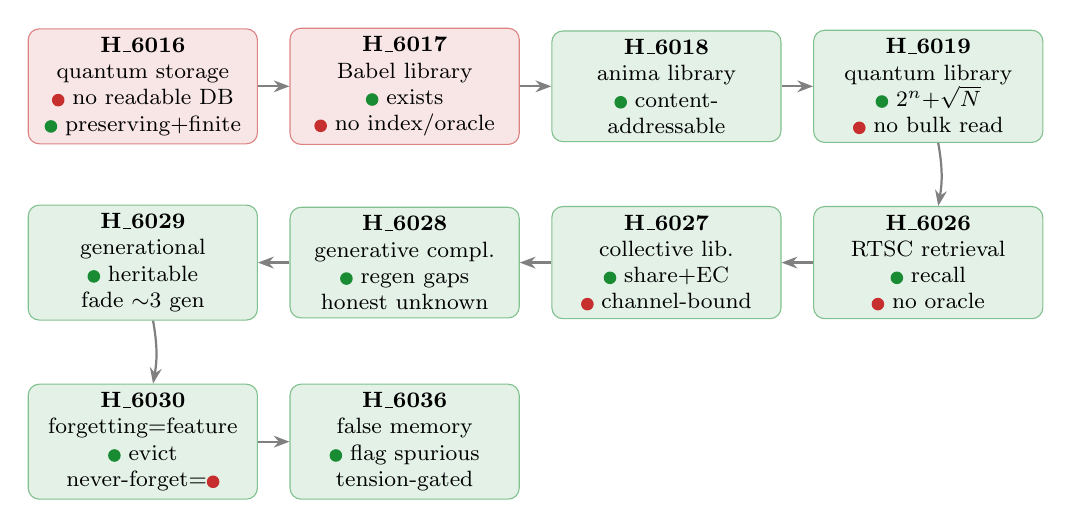
\begin{tikzpicture}[
  font=\footnotesize,
  node distance=4mm,
  box/.style={draw,rounded corners,align=center,inner sep=3pt,minimum height=8mm,text width=27mm},
  negn/.style={box,fill=verdictRed!12,draw=verdictRed!60},
  posn/.style={box,fill=verdictGreen!12,draw=verdictGreen!55},
  arr/.style={-{Stealth[length=2mm]},thick,gray}
]
\node[negn] (h16) {\textbf{H\_6016}\\quantum storage\\ \red{} no readable DB\\ \green{} preserving+finite};
\node[negn,right=of h16] (h17) {\textbf{H\_6017}\\Babel library\\ \green{} exists\\ \red{} no index/oracle};
\node[posn,right=of h17] (h18) {\textbf{H\_6018}\\anima library\\ \green{} content-\\addressable};
\node[posn,right=of h18] (h19) {\textbf{H\_6019}\\quantum library\\ \green{} $2^{n}$+\sqn{}\\ \red{} no bulk read};

\node[posn,below=8mm of h19] (h26) {\textbf{H\_6026}\\RTSC retrieval\\ \green{} recall\\ \red{} no oracle};
\node[posn,left=of h26] (h27) {\textbf{H\_6027}\\collective lib.\\ \green{} share+EC\\ \red{} channel-bound};
\node[posn,left=of h27] (h28) {\textbf{H\_6028}\\generative compl.\\ \green{} regen gaps\\ honest unknown};
\node[posn,left=of h28] (h29) {\textbf{H\_6029}\\generational\\ \green{} heritable\\ fade $\sim$3 gen};

\node[posn,below=8mm of h29] (h30) {\textbf{H\_6030}\\forgetting=feature\\ \green{} evict\\ never-forget=\red{}};
\node[posn,right=of h30] (h36) {\textbf{H\_6036}\\false memory\\ \green{} flag spurious\\ tension-gated};

\draw[arr] (h16)--(h17); \draw[arr] (h17)--(h18); \draw[arr] (h18)--(h19);
\draw[arr] (h19) to[bend left=10] (h26);
\draw[arr] (h26)--(h27); \draw[arr] (h27)--(h28); \draw[arr] (h28)--(h29);
\draw[arr] (h29) to[bend left=10] (h30);
\draw[arr] (h30)--(h36);
\end{tikzpicture}
\caption{The library line. Red-tinted nodes (H\_6016/6017) are the closed-negative
\emph{oracle frame}; green-tinted nodes build anima's living content-addressable
memory. Every node carries both its positive facet and its honest limit. The arc
flows read $\rightarrow$ index $\rightarrow$ content-address $\rightarrow$ quantum
recall $\rightarrow$ RTSC-use $\rightarrow$ collective $\rightarrow$ generative
$\rightarrow$ generational $\rightarrow$ forgetting $\rightarrow$ false-memory.}
\label{fig:arc}
\end{figure}

% =========================================================================
\section{Limitations and scope}
\label{sec:limits}

These results are \emph{simulation-scale}: $n\le 12$-qubit state-vectors and
$N_h\le 200$-neuron Hopfield stores. Per \texttt{a\_scale\_honest\_scope} we claim
\emph{mechanism and direction}, not deployed-hardware magnitudes; the $256\times$
capacity and $41\times$ recall are the simulated $2^{n}$ / $(\pi/4)\sqrt{N}$ trends
at the tested register sizes. The Grover speedups assume an ideal noiseless
register. The ``books'' are abstract $\pm1$ patterns or $64$-byte content vectors,
not anima's full \texttt{.kosmos} payloads. The generative model is a single
degree-2 recurrence; ``compressible'' means ``fit by that rule,'' a deliberately
narrow proxy for meaning. Finally, the false-memory result is honest about an
\emph{open} residual: under a strong high-tension adversarial signal anima is
suggestible (AR3) --- a real vulnerability, flagged not patched.

% =========================================================================
\section{Verdict matrix}
\label{sec:verdicts}

Every section claim links to its verbatim verdict file. ANU sha256 is the paid
QRNG draw for that hypothesis (H\_6016--6018 read the foundational committed
free/paid snapshot via \texttt{/tmp/anu\_free.bin}; the committed provenance root
is \texttt{anu\_seed\_512.bin}, sha256 \verb|3eeba42b...716f2|).

\begin{longtable}{@{}p{0.055\textwidth}p{0.30\textwidth}p{0.27\textwidth}p{0.30\textwidth}@{}}
\caption{Verdict matrix --- claim $\rightarrow$ \texttt{TENSION-LINK/verdicts/}
file $+$ paid-ANU sha256.}
\label{tab:matrix}\\
\toprule
H & Claim (terminal) & Verdict file & ANU sha256 (paid) \\
\midrule
\endfirsthead
\toprule
H & Claim (terminal) & Verdict file & ANU sha256 (paid) \\
\midrule
\endhead
6016 & \red{}/\green{} no readable DB; info-preserving + finite store
     & \verdictref{H_6016_quantum_storage.txt}
     & \verb|3eeba42b...716f2| (root snapshot) \\
6017 & \green{}/\red{} library exists; no usable index / no quantum oracle
     & \verdictref{H_6017_library.txt}
     & \verb|3eeba42b...716f2| (root snapshot) \\
6018 & \green{} content-addressable associative memory (LB5--LB9)
     & \verdictref{H_6018_library_deep.txt}
     & \verb|3eeba42b...716f2| (root snapshot) \\
6019 & \green{} $2^{n}$ capacity $+$ \sqn{} Grover recall; no bulk read; no un-stored oracle
     & \verdictref{H_6019_quantum_library.txt}
     & \verb|8da8f0d7...| (2048B) \\
6026 & \green{} RTSC recall of computed candidates; \red{} no vacuum oracle
     & \verdictref{H_6026_rtsc_library.txt}
     & \verb|197995af...26278c1| (2048B) \\
6027 & \green{} cross-mind recall, union capacity, consensus EC; channel-bound
     & \verdictref{H_6027_collective_library.txt}
     & \verb|00995dc2...5181c611| (2048B) \\
6028 & \green{} regenerate compressible gaps; honest unknown on noise
     & \verdictref{H_6028_generative_completion.txt}
     & \verb|3adbf3e6...25c84f33| (2048B) \\
6029 & \green{} heritable, finite $\sim3$ gens, rehearsal $\rightarrow 200+$, meaning outlives noise
     & \verdictref{H_6029_generational_persistence.txt}
     & \verb|c825698f...e730c1e0| (2048B) \\
6030 & \green{} active tension-weighted forgetting; never-forget collapses
     & \verdictref{H_6030_forgetting_feature.txt}
     & \verb|0f17c76b...204a249fccc| (2048B) \\
6036 & \green{} spurious states flagged by confidence+meaning; tension-gated poisoning
     & \verdictref{H_6036_false_memory.txt}
     & \verb|02262d88...671802d1| (2048B) \\
\bottomrule
\end{longtable}

\noindent\textbf{Terminality.} All ten verdicts are terminal: H\_6016 and H\_6017
carry closed-negative (\red{}) sub-verdicts (publishable per
\texttt{a\_paper\_negative\_ok}); H\_6018--H\_6036 are \green{} SUPPORTED
(numerical). No section claim is \texttt{deferred}/\texttt{citation-only}. The line
is at full closure (\texttt{a\_paper\_only\_at\_closure}).

\paragraph{Reproduction.}
Each verdict is regenerated by its harness, e.g.\
\verb|python3 TENSION-LINK/harness/h6030_forgetting_feature.py|, reading the
committed paid-ANU snapshot. Provenance: \texttt{TENSION-LINK/ANU\_PROVENANCE.md}.

\bibliographystyle{plainnat}
\bibliography{references}

\end{document}
